\documentclass[9pt]{article}
\usepackage{graphicx} % Required for inserting images
\usepackage{tabularx}
\usepackage{hyperref}
\usepackage{makecell}
\usepackage{makeidx}
\usepackage{eurosym}
\usepackage{fancyhdr}
\usepackage{titlesec}
\usepackage[export]{adjustbox}
\usepackage{float}
\newcommand{\firstPage}{
    \thispagestyle{empty}
    \begin{figure}
    \centering
    
\includegraphics[scale=0.7]{Swellfish_logo.png}
    \end{figure}
    \author{
        \date{}
        \href{mailto://swellfish14@gmail.com}{swellfish14@gmail.com} \\
    } 
} 
\usepackage{hyperref}
\usepackage{array}
\usepackage{tabularx}
\usepackage{adjustbox}

\newcounter{verscount}
\setcounter{verscount}{0}
\newcommand{\addversione}[5]{
	\ifdefined\setversione
		\setversione{#1}
	\else\fi
	\stepcounter{verscount}
	\expandafter\newcommand%
		\csname ver\theverscount \endcsname{#1&#2&#3&#4&#5}
}

\newcommand{\listversioni}{
	\ifnum\value{verscount}>1
		\csname ver\theverscount \endcsname
		\addtocounter{verscount}{-1}
		\\\hline
		\listversioni
	\else
		\csname ver\theverscount \endcsname\\\hline
	\fi
}

\newcommand{\makeversioni}{
	\begin{center}
		\begin{tabularx}{\textwidth}{|c|c|X|X|X|}
		\hline
		\textbf{Versione} & \textbf{Data} & \textbf{Redattore} & \textbf{Verificatore} & \textbf{Descrizione} \\
		\hline
		\listversioni
		\end{tabularx}
	\end{center}
	\clearpage
}

\fancypagestyle{genericDocstyle}{
	\pagestyle{fancy}
	\lhead{
\includegraphics[width=1cm]{Swellfish_logo.png}}
	\rhead{Norme di progetto}
}

%\hypersetup{colorlinks=true,urlcolor=blue}

%\newcommand{\tableContent}{

	%{
		%\hypersetup{linkcolor=black}
		%\tableofcontents
	%}
%}

\begin{document}
\graphicspath{ {../templates/img/} {./img}}
\setcounter{tocdepth}{4}
\setcounter{secnumdepth}{4}
\title{Manuale Utente}

\firstPage
\maketitle

\begin{center}
	\begin{tabular}{r | l}
		\multicolumn{2}{c}{\textit{Informazioni}}                         \\
		\hline

		\textit{Redattori}    &
		[Claudio Giaretta, Francesco Naletto]\makecell{} \\

		\textit{Revisori}     &
		[Jude Vensil Barceros]\makecell{}                                 \\
		\textit{Responsabili} &
		[Andrea Veronese]\makecell{}                                      \\
		\textit{Uso}          &
		[Esterno]\makecell{}                                              \\
	\end{tabular}
\end{center}

\begin{center}
	\textbf{Descrizione}\\
	File contenente Questo documento racchiude le istruzioni per l’utilizzo corretto di LumosMinima
\end{center}

\pagebreak

\printindex
\pagebreak

\tableofcontents
\pagebreak

\addversione{0.0.0}{23/08/2023}{Davide Porporati}{Claudio Giaretta}{Impostata struttura documento}

\makeversioni

\section{Introduzione}
\section{Strumenti necessari}
\section{LumosMinima}
\subsection{Home}
Il sito LumosMinima si presenta con una dashboard composta di 4 pannelli che danno informazioni generali 
sul sistema

\begin{center}
	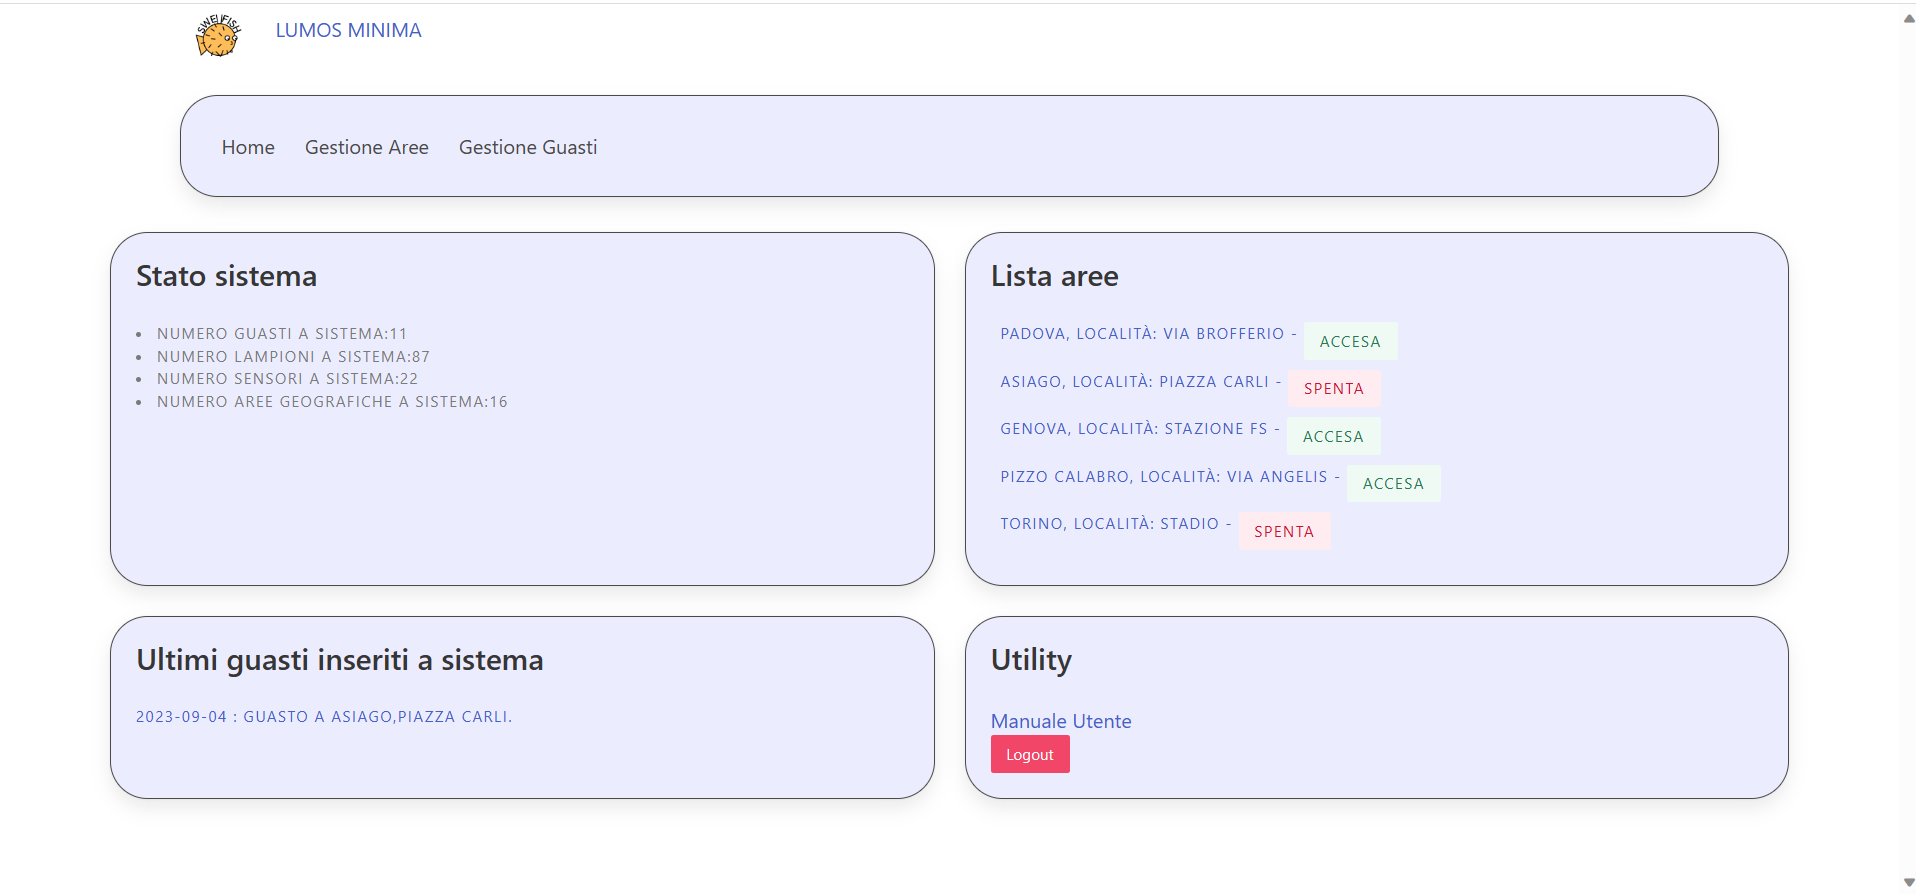
\includegraphics[scale=0.3]{LumosMinimaHome.png}
\end{center}

In particolare:
\begin{itemize}
	\item \textbf{la sezione 1}: indica informazioni riguardanti lo stato del sistema
	\item \textbf{la sezione 2}: riporta una lista delle ultime 9 segnalazioni di guasti inseriti a sistema dall'utente
	\item \textbf{la sezione 3}: riporta una lista delle aree illuminate inserite a sistema
	\item \textbf{la sezione 4}: riporta un link in cui è possibile scaricare il manuale utente\\
\end{itemize}

La navbar presente in alto (sezione 5) è composta da 3 link:

\begin{itemize}
\item \textbf{Home}: Porta alla pagina corrente ovvero la Home
\item \textbf{Gestione aree}: porta alla pagina "Gestione Aree" in cui è possibile gestire le varie aree inserite a sistema
\item \textbf{Gestione guasti}: porta alla pagina in cui vengono visualizzati tutti i guasti segnalati a sistema
\end{itemize}

\subsection{Gestione aree}
In questa pagina è presente la lista di tutte le aree inserite a sistema. 
Ogni area è rappresentata da un link cliccabile che porta alla pagina di dettaglio corrispondente all'area cliccata.

\begin{center}
	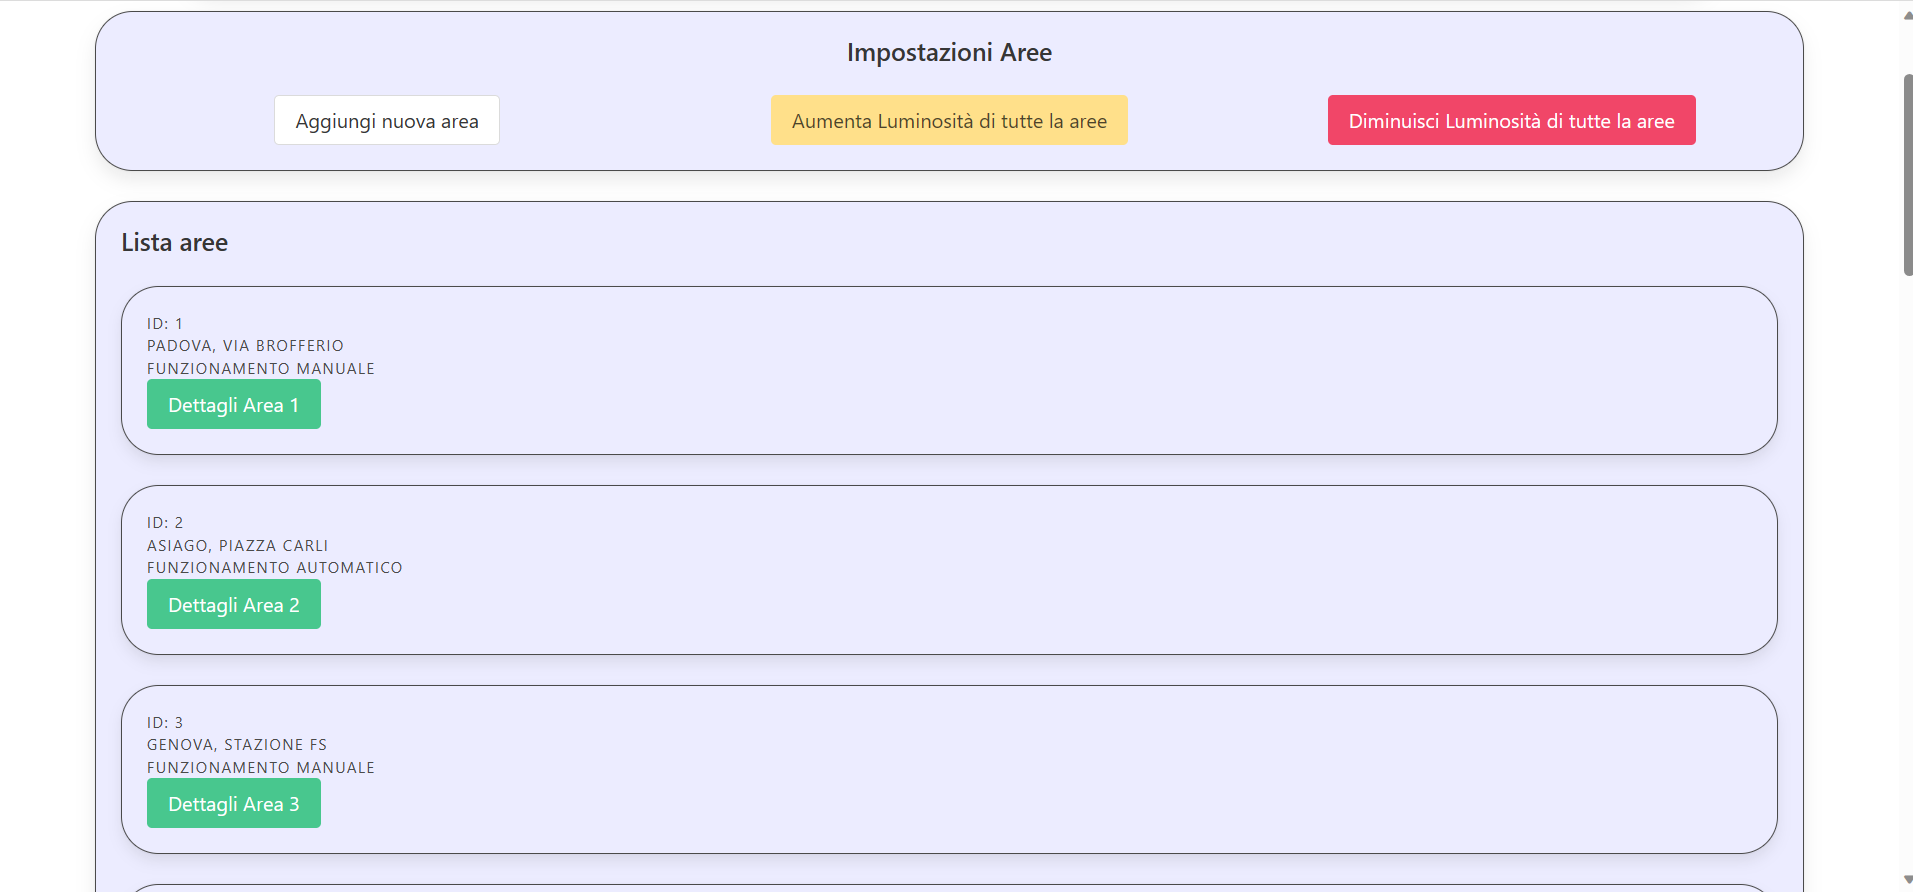
\includegraphics[scale=0.3]{Gestione_aree.png}
\end{center}

Nella sezione 2 è presente il tasto per aggiungere una nuova area di illuminazione, che porterà alla pagina "Aggiugni area". 

\subsection{Aggiungi area}

In questa pagina è possibile immettere tutte le informazioni riguardanti l'area illuminata che si vuole inserire.

\begin{center}
	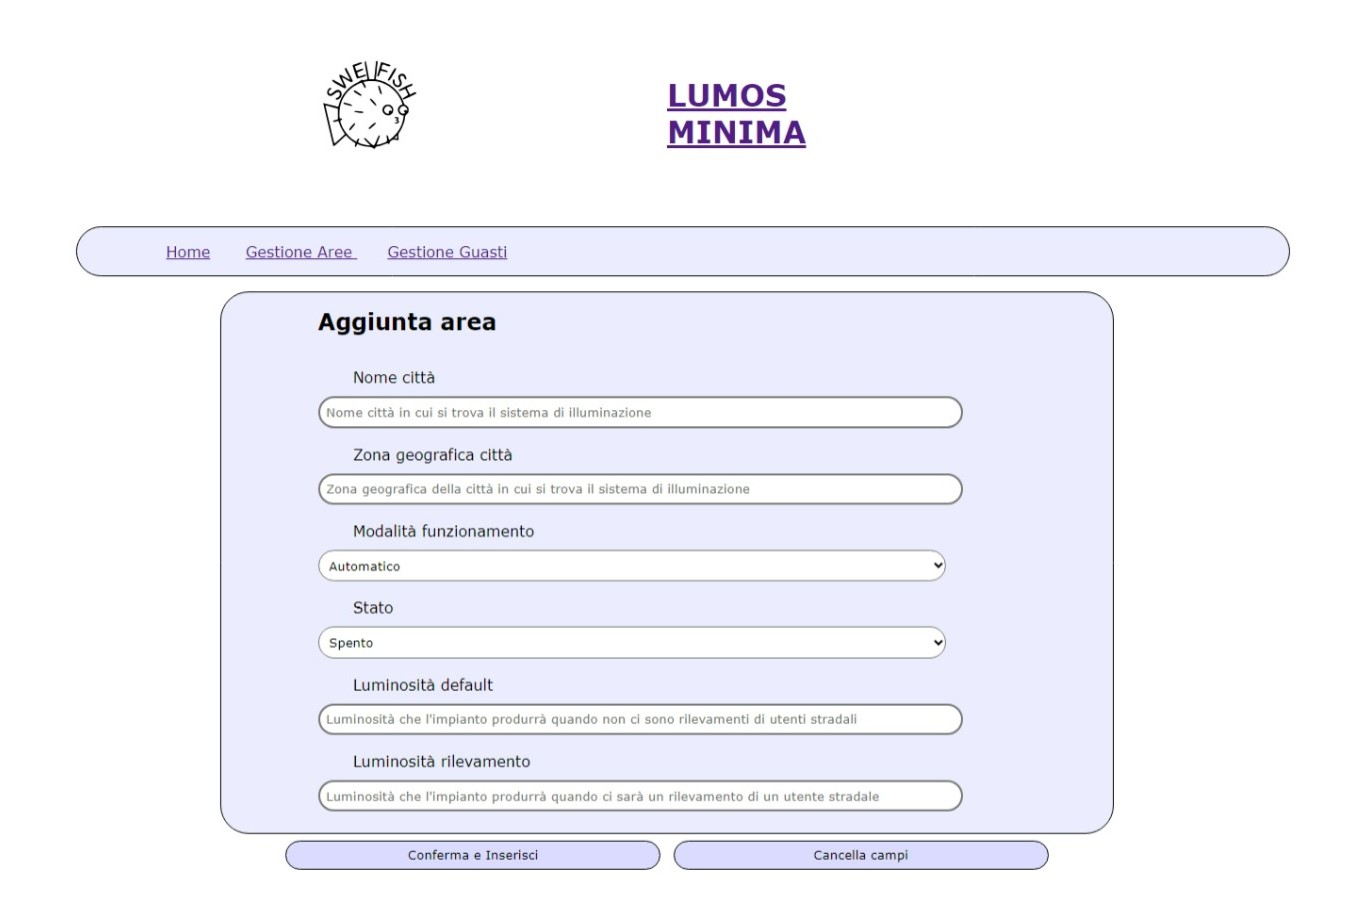
\includegraphics[scale=0.3]{Aggiungi_area.png}
\end{center}	

Una volta terminato l'inserimento dei dati, cliccando sul pulsante "Conferma e Inserisci" 
l'area verrà inserita nel sistema e si verrà reindirizzati nella pagina "Area" con il dettaglio dell'area appena inserita.

\subsection{Area}

In questa area è possibile gestire tutti gli aspetti legati all'area di illuminazione selezionata

\begin{center}
	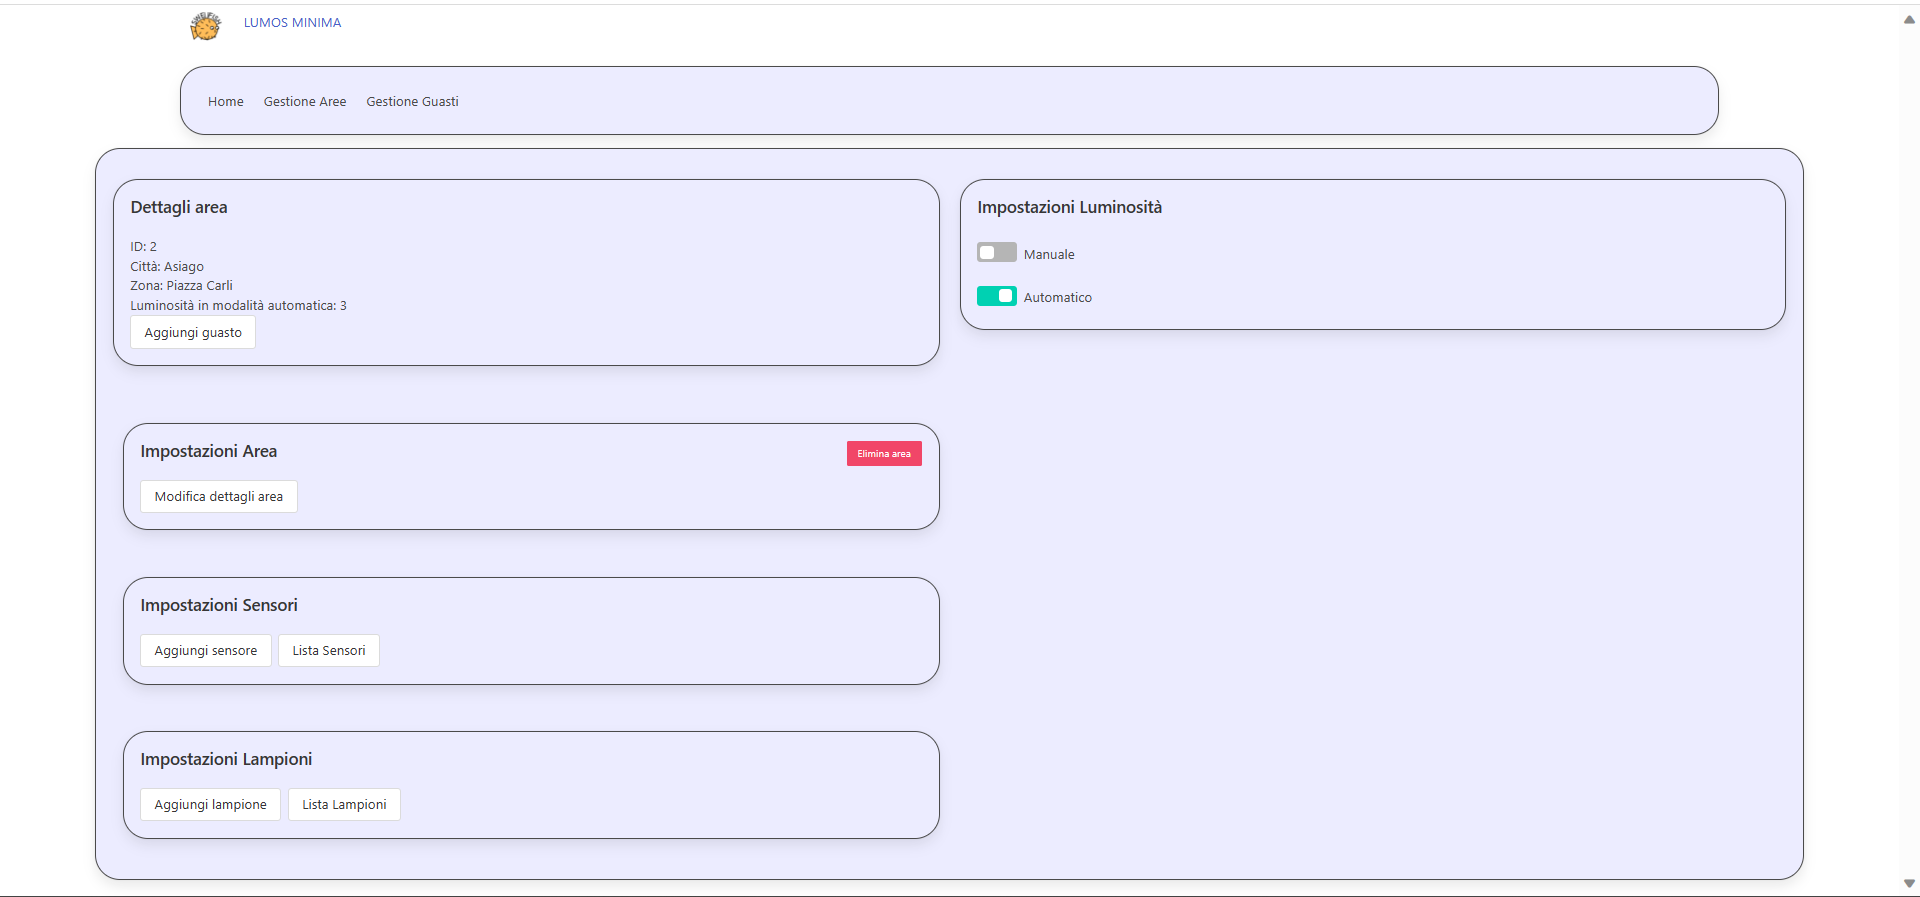
\includegraphics[scale=0.3]{Area.png}
\end{center}	

La pagina è suddivisa nei seguenti riquadri:
\begin{itemize}
	\item \textbf{la sezione 1}: Informazioni contententi i dettagli dell'area, è presente un pulsante con cui è possibile spegnere o accendere tutta l'area
	\item \textbf{la sezione 2}: Contiene i pulsanti che permettono di eliminare o modificare l'area.
	\item \textbf{la sezione 3}: 
	\item \textbf{la sezione 4}: 
\end{itemize}
\subsection{Gestione guasti}

\subsection{Aggiungi area}
\subsection{Aggiungi lampione}
\subsection{Aggiungi sensore}

\end{document}
